\chapter{Основные теоретические сведения}
Программа PCLAB предназначена для исследования производительности x86 совместимых ЭВМ c IA32 архитектурой, работающих под управлением операционной системы Windows (версий 95 и старше). Исследование организации ЭВМ заключается в проведении ряда экспериментов, направленных на построение зависимостей времени обработки критических участков кода от изменяемых параметров. Набор реализуемых программой экспериментов позволяет исследовать особенности построения современных подсистем памяти ЭВМ и процессорных устройств, выявить конструктивные параметры конкретных моделей ЭВМ. 

Процесс сбора и анализа экспериментальных данных в PCLAB основан на процедуре профилировки критического кода, т.е. в измерении времени его обработки центральным процессорным устройством. При исследовании конвейерных суперскалярных процессорных устройств, таких как 32-х разрядные процессоры фирмы Intel или AMD, способных выполнять переупорядоченную обработку последовательности команд программы, требуется использовать специальные средства измерения временных интервалов и запрещения переупорядочивания микрокоманд. 

\chapter{Экспериментальная часть}


\section*{Эксперимент №1: Исследования расслоения динамической памяти}
\addcontentsline{toc}{section}{Эксперимент №1}

\subsection*{Цель эксперимента}
Определение способа трансляции физического адреса, используемого при обращении к динамической памяти. 

\subsection*{Описание проблемы}
В связи с конструктивной неоднородностью оперативной памяти, обращение к последовательно расположенным данным требует различного времени. В связи с этим, для создания эффективных программ необходимо учитывать расслоение памяти, характеризуемое способом трансляции физического адреса.

\subsection*{Исходные данные}
Размер линейки кэш-памяти верхнего уровня; объем физической памяти.

\clearpage

\subsection*{Результаты эксперимента}
На рисунке \ref{ex:t1} представлен график, полученный в результате эксперимента с исходными параметрами:
\begin{itemize}
	\item Максимальное расстояния между	читаемыми блоками (К) = 32;
	\item Шаг увеличения расстояния между читаемыми 4-х байтовыми ячейками (Б) = 64;
	\item Размер массива (М) = 4.
\end{itemize}

\begin{figure}[h]
	\centering
	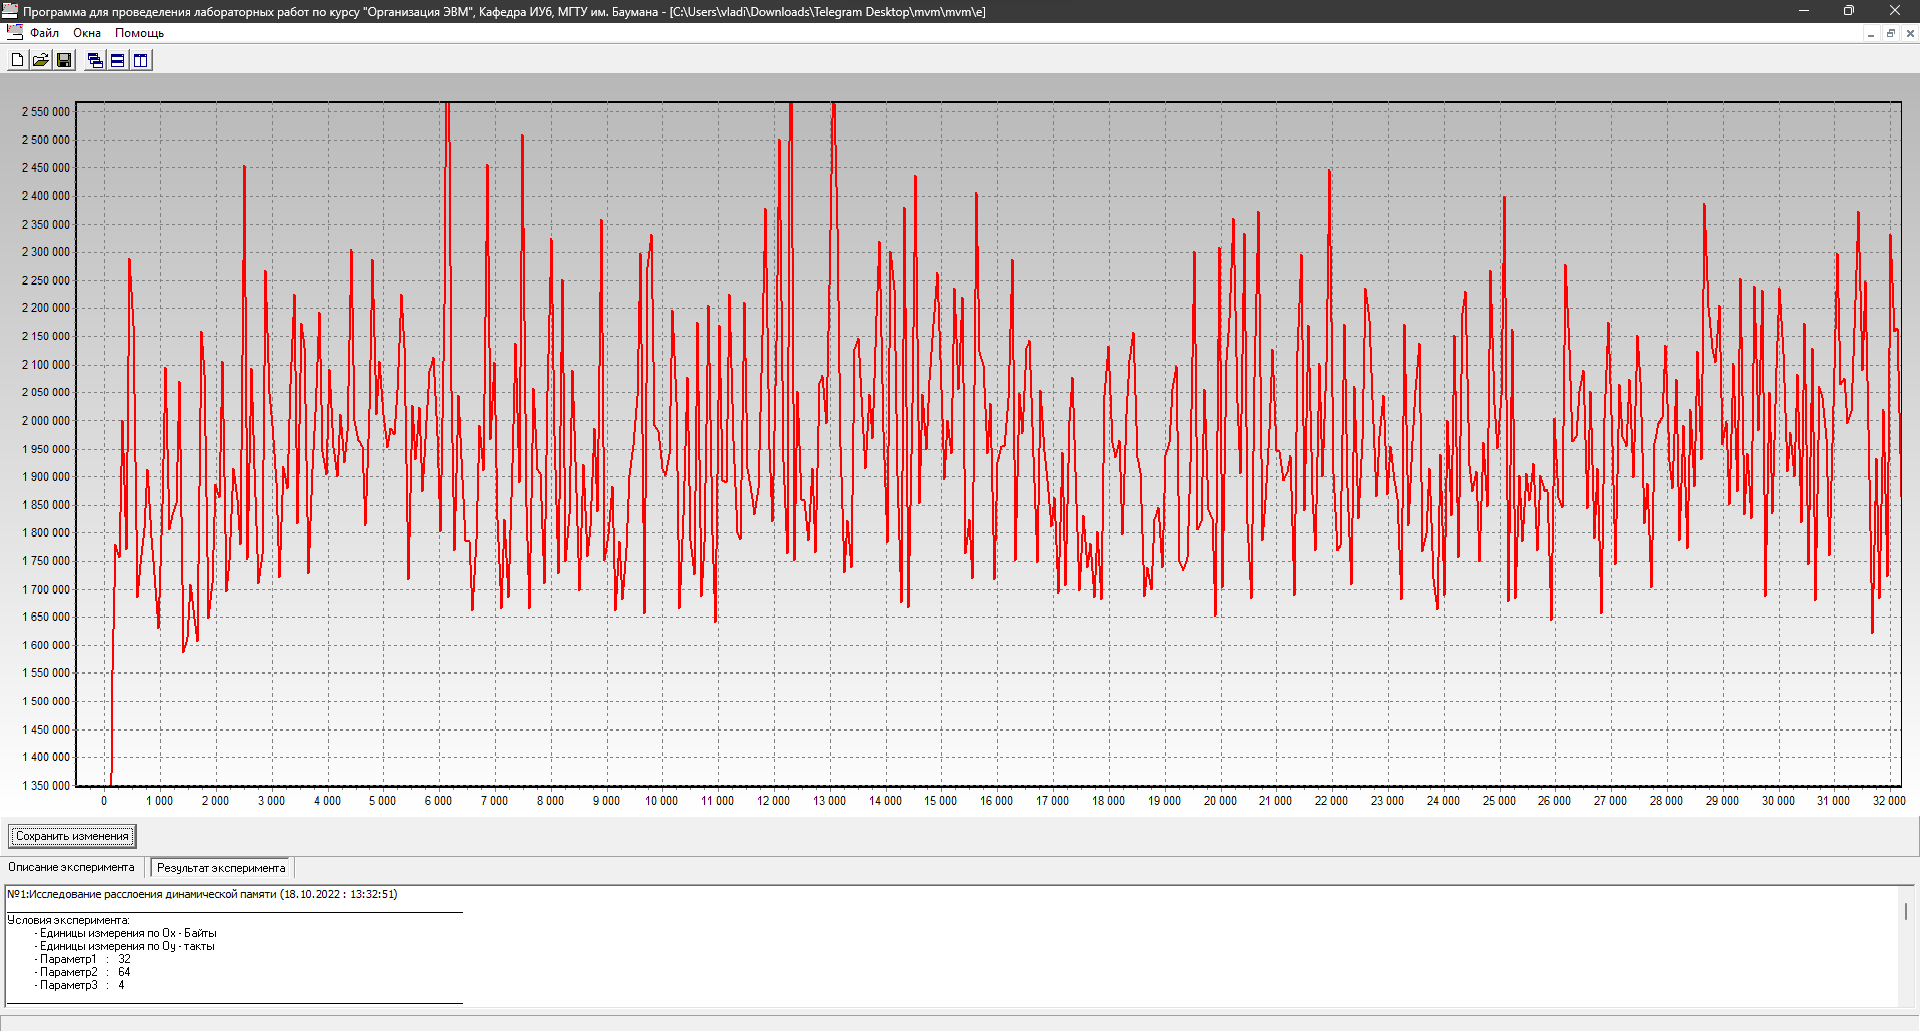
\includegraphics[height=0.35\textheight]{img/t1}
	\caption{Эксперимент №1: Исследования расслоения динамической памяти}
	\label{ex:t1}
\end{figure}

Первый пик, который мы видим на рисунке \ref{ex:t1} -- адресное расстояние между страницей в одном банке и следующей страницей в том же банке. Это адресное расстояние равно 1024.

\newpage

\subsection*{Вывод}
Оперативная память неоднородна, и для обращения к последовательно расположенными данным может потребоваться различное количество времени. Поэтому, при создании программ необходимо учитывать расслоение памяти при обработке данных.

\newpage


\section*{Эксперимент №2: Сравнение эффективности ссылочных и векторных структур}
\addcontentsline{toc}{section}{Эксперимент №2}

\subsection*{Цель эксперимента}
Оценка влияния зависимости команд по данным на эффективность вычислений. 

\subsection*{Описание проблемы}
Обработка зависимых данных происходит в тех случаях, когда результат работы одной команды используется в качестве адреса операнда другой. При программировании на языках высокого уровня такими операндами являются указатели, активно используемые при обработке ссылочных структур данных: списков, деревьев, графов. Обработка данных структур процессорами с длинными конвейерами команд приводит к заметному увеличению времени работы алгоритмов: адрес загружаемого операнда становится известным только после обработки предыдущей команды. В противоположность этому, обработка векторных структур, таких как массивы, позволяет эффективно использовать аппаратные возможности ЭВМ. 

\subsection*{Результаты эксперимента}
На рисунке \ref{ex:t2} представлен график, полученный в результате эксперимента с исходными параметрами:
\begin{itemize}
	\item Количество элементов в списке (М) = 5;
	\item Максимальная фрагментации списка (К) = 400;
	\item Шаг увеличения фрагментации (К) = 7.
\end{itemize}

\begin{figure}[h]
	\centering
	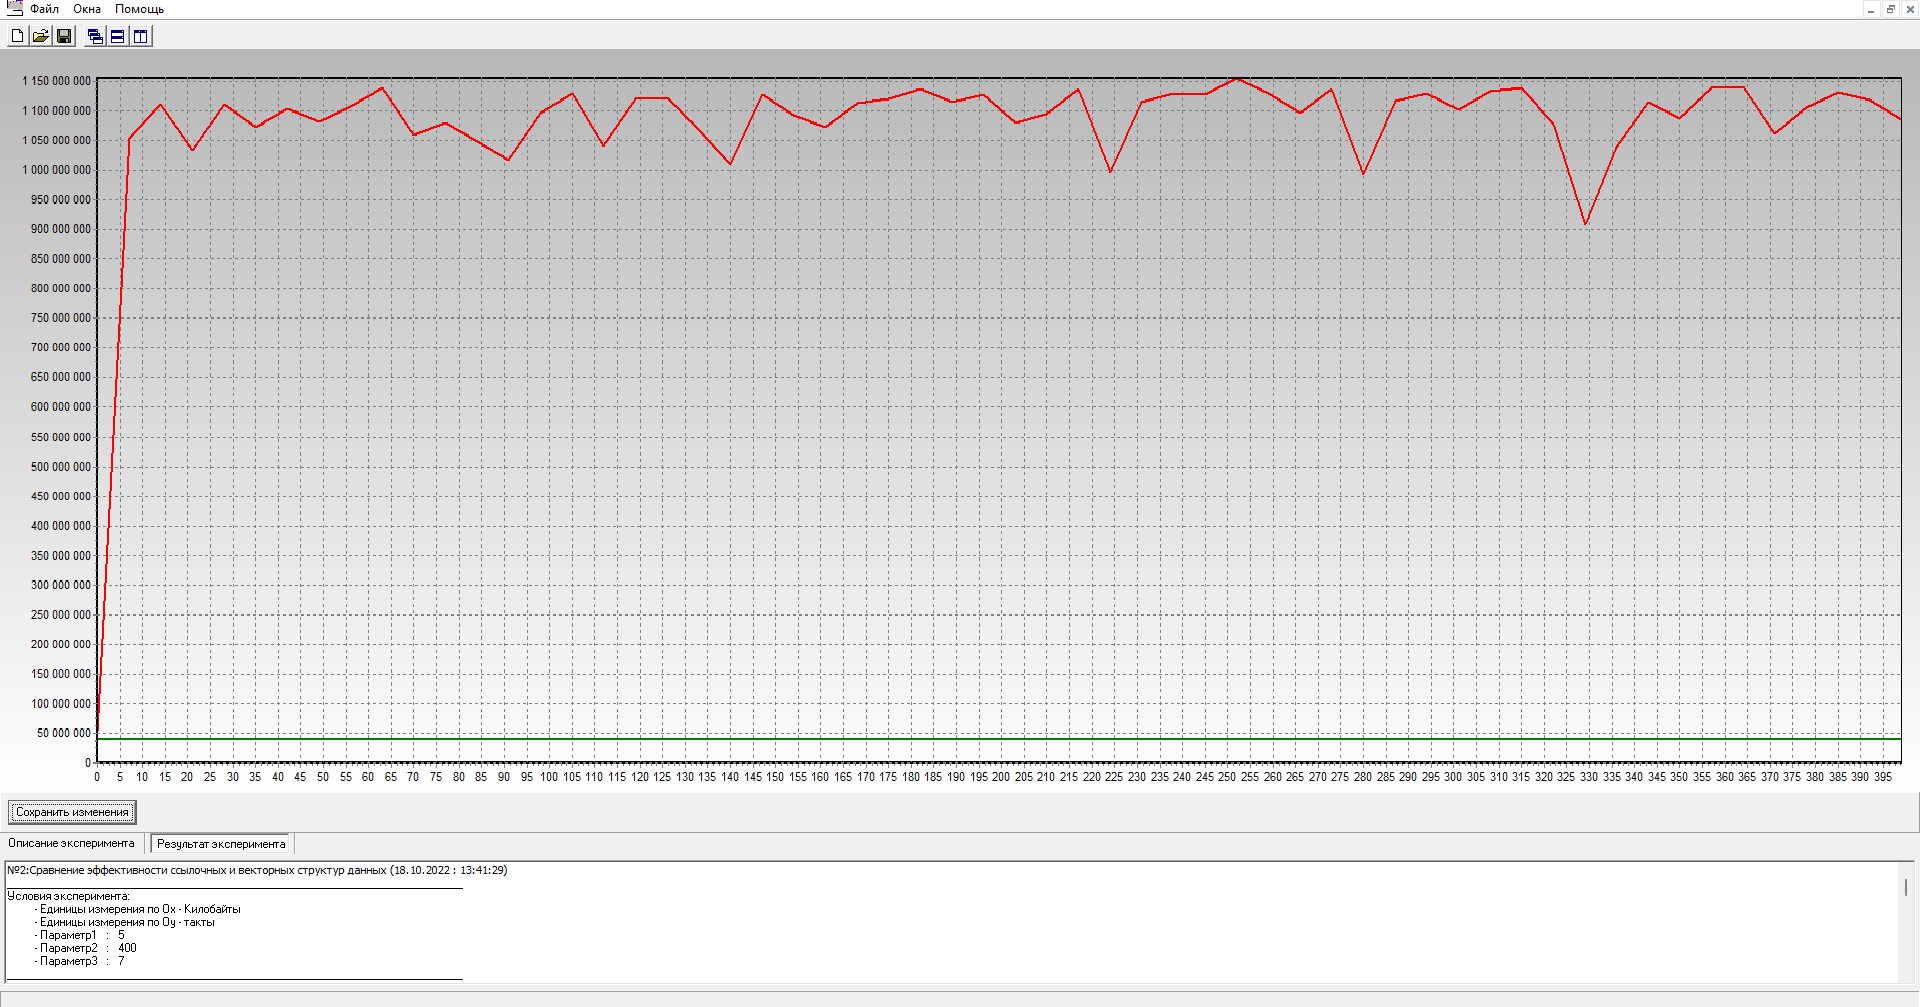
\includegraphics[height=0.35\textheight]{img/t2}
	\caption{Эксперимент №2: Сравнение эффективности ссылочных и векторных структур}
	\label{ex:t2}
\end{figure}

Результат сравнения времени (как вывод программы) представлен на рисунке \ref{ex:t2-data}. Как видно на рисунке, список обрабатывается почти в 20-30 раз медленнее.

\begin{figure}[h]
	\centering
	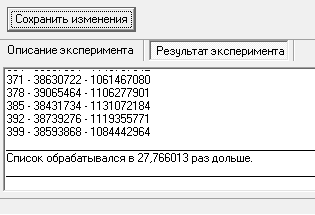
\includegraphics[height=0.25\textheight]{img/t2-data}
	\caption{Эксперимент №2: Результат}
	\label{ex:t2-data}
\end{figure}

\newpage

\subsection*{Вывод}
Вывод из полученных результатов можно сделать следующий: использовать структуры данных надо с учетом технологического фактора определенной задачи. Если решаемая задача предполагает возможность использования массива, то надо использовать его, особенно если использование списка не дает существенной разницы (особенно выигрыша во времени).

\newpage

\section*{Эксперимент №3: Исследование эффективности программной предвыборки}
\addcontentsline{toc}{section}{Эксперимент №3}

\subsection*{Цель эксперимента}
Выявление способов ускорения вычислений благодаря применению предвыборки данных. 

\subsection*{Исходные данные}
Степень ассоциативности и размер TLB данных.

\subsection*{Описание проблемы}
Обработка больших массивов информации сопряжена с открытием большого количества физических страниц памяти. При первом обращении к странице памяти наблюдается увеличенное время доступа к данным. Это связано с необходимостью преобразования логического адреса в физический адрес памяти, а также c открытием страницы динамической памяти и сохранения данных в кэш-памяти.

Преобразование выполняется на основе информации о использованных ранее страницах, содержащейся в TLB буфере процессора. Первое обращение к странице при отсутствии информации в TLB вызывает двойное обращение к оперативной памяти: сначала за информацией из таблицы страниц, а далее за востребованными данными. Предвыборка заключается в заблаговременном проведении всех указанных действий благодаря дополнительному запросу небольшого количества данных из оперативной памяти. 

\subsection*{Результаты эксперимента}

На рисунке \ref{ex:t3} представлен график, полученный в результате эксперимента с исходными параметрами:
\begin{itemize}
	\item Шаг увеличения расстояния между читаемыми данными (Б) = 256;
	\item Размер массива (К) = 128.
\end{itemize}

\begin{figure}[h]
	\centering
	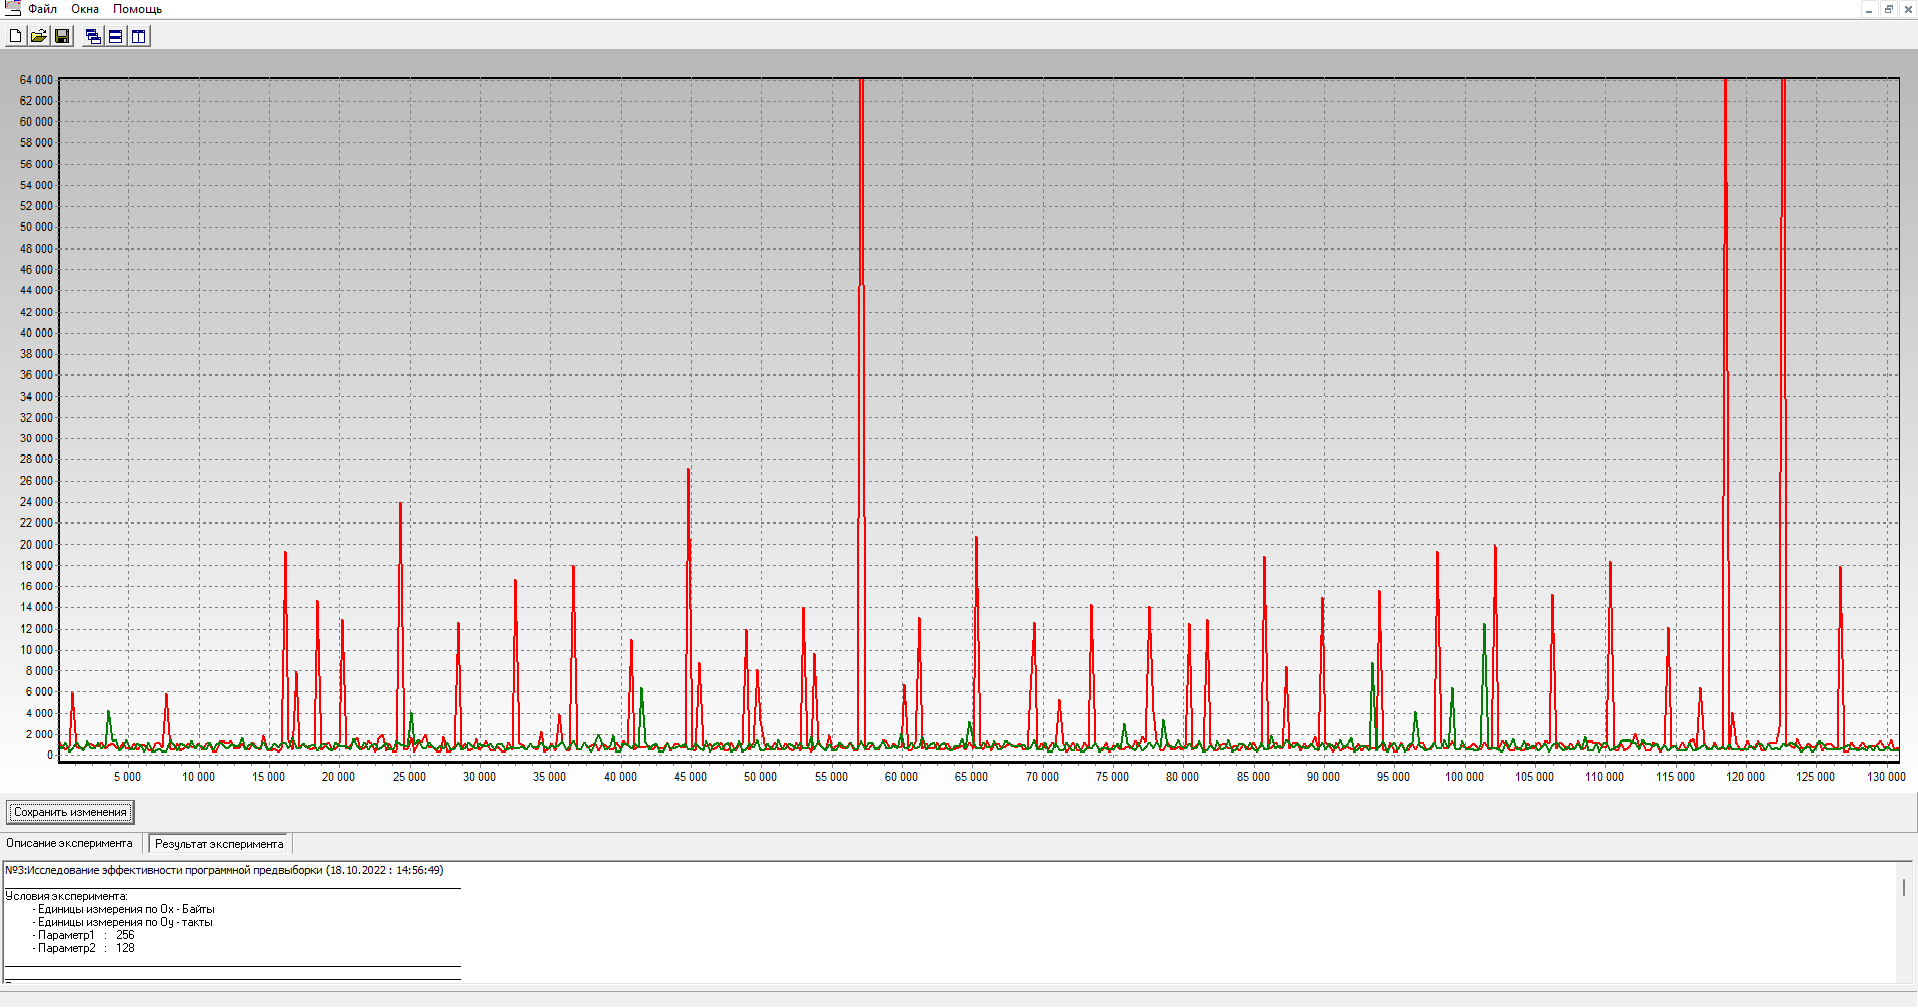
\includegraphics[height=0.35\textheight]{img/t3}
	\caption{Эксперимент №3: Исследование эффективности программной предвыборки}
	\label{ex:t3}
\end{figure}

Результат сравнения времени (как вывод программы) представлен на рисунке \ref{ex:t3-data}. Как видно на рисунке, обработка без загрузки таблицы страниц в TLB производилась в 2,454523 раз дольше.

\begin{figure}[h]
	\centering
	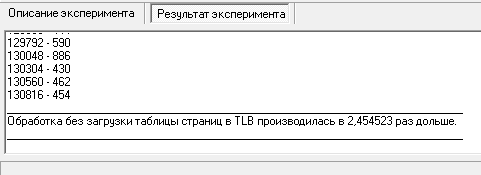
\includegraphics[height=0.15\textheight]{img/t3-data}
	\caption{Эксперимент №3: Результат}
	\label{ex:t3-data}
\end{figure}

Красный график - чтение страниц последовательно из оперативной памяти. Зеленый график - чтение страниц, используя дополнительный цикл предвыборки, обеспечивающий своевременную загрузку информации в TLB данных.

Сокращение времени работы алгоритма, который использует предвыборку, происходит в том случае, когда информация о востребованных страницах помещается в TLB. 

Пики на красном графике происходят из-за того, что процессу неободимо преобразовать физический адрес в логический.

\subsection*{Вывод}
Используя предвыборку можно ускорить время работы программы почти в 2 раза (как результат представлен 2.4) за счет заблаговременной загрузки страниц в память.

\newpage

\section*{Эксперимент №4: Исследование способов эффективного чтения оперативной памяти}
\addcontentsline{toc}{section}{Эксперимент №4}

\subsection*{Цель эксперимента}
Исследование возможности ускорения вычислений благодаря использованию структур данных, оптимизирующих механизм чтения оперативной памяти.

\subsection*{Исходные данные}
Адресное расстояние между банками памяти, размер буфера чтения.

\subsection*{Описание проблемы}
При обработке информации, находящейся в нескольких страницах и банках оперативной памяти возникают задержки, связанные с необходимостью открытия и закрытия страниц DRAM памяти. При программировании на языках высокого уровня такая ситуация наблюдается при интенсивной обработке нескольких массивов данных или обработке многомерных массивов. При этом процессоры, в которых реализованы механизмы аппаратной предвыборки, часто не могут организовать эффективную загрузку данных. Кроме этого, объемы запрошенных данных оказываются заметно меньше размера пакета, передаваемого из оперативной памяти. Таким образом, эффективная обработка нескольких векторных структур данных без их дополнительной оптимизации не использует в должной степени возможности аппаратных ресурсов. 

\subsection*{Результаты эксперимента}
На рисунке \ref{ex:t3} предаставлен график, полученный в результате эксперимента с исходными параметрами:
\begin{itemize}
	\item Размер массива (М) = 2;
	\item Количество потоков данных = 64.
\end{itemize}

\begin{figure}[h]
	\centering
	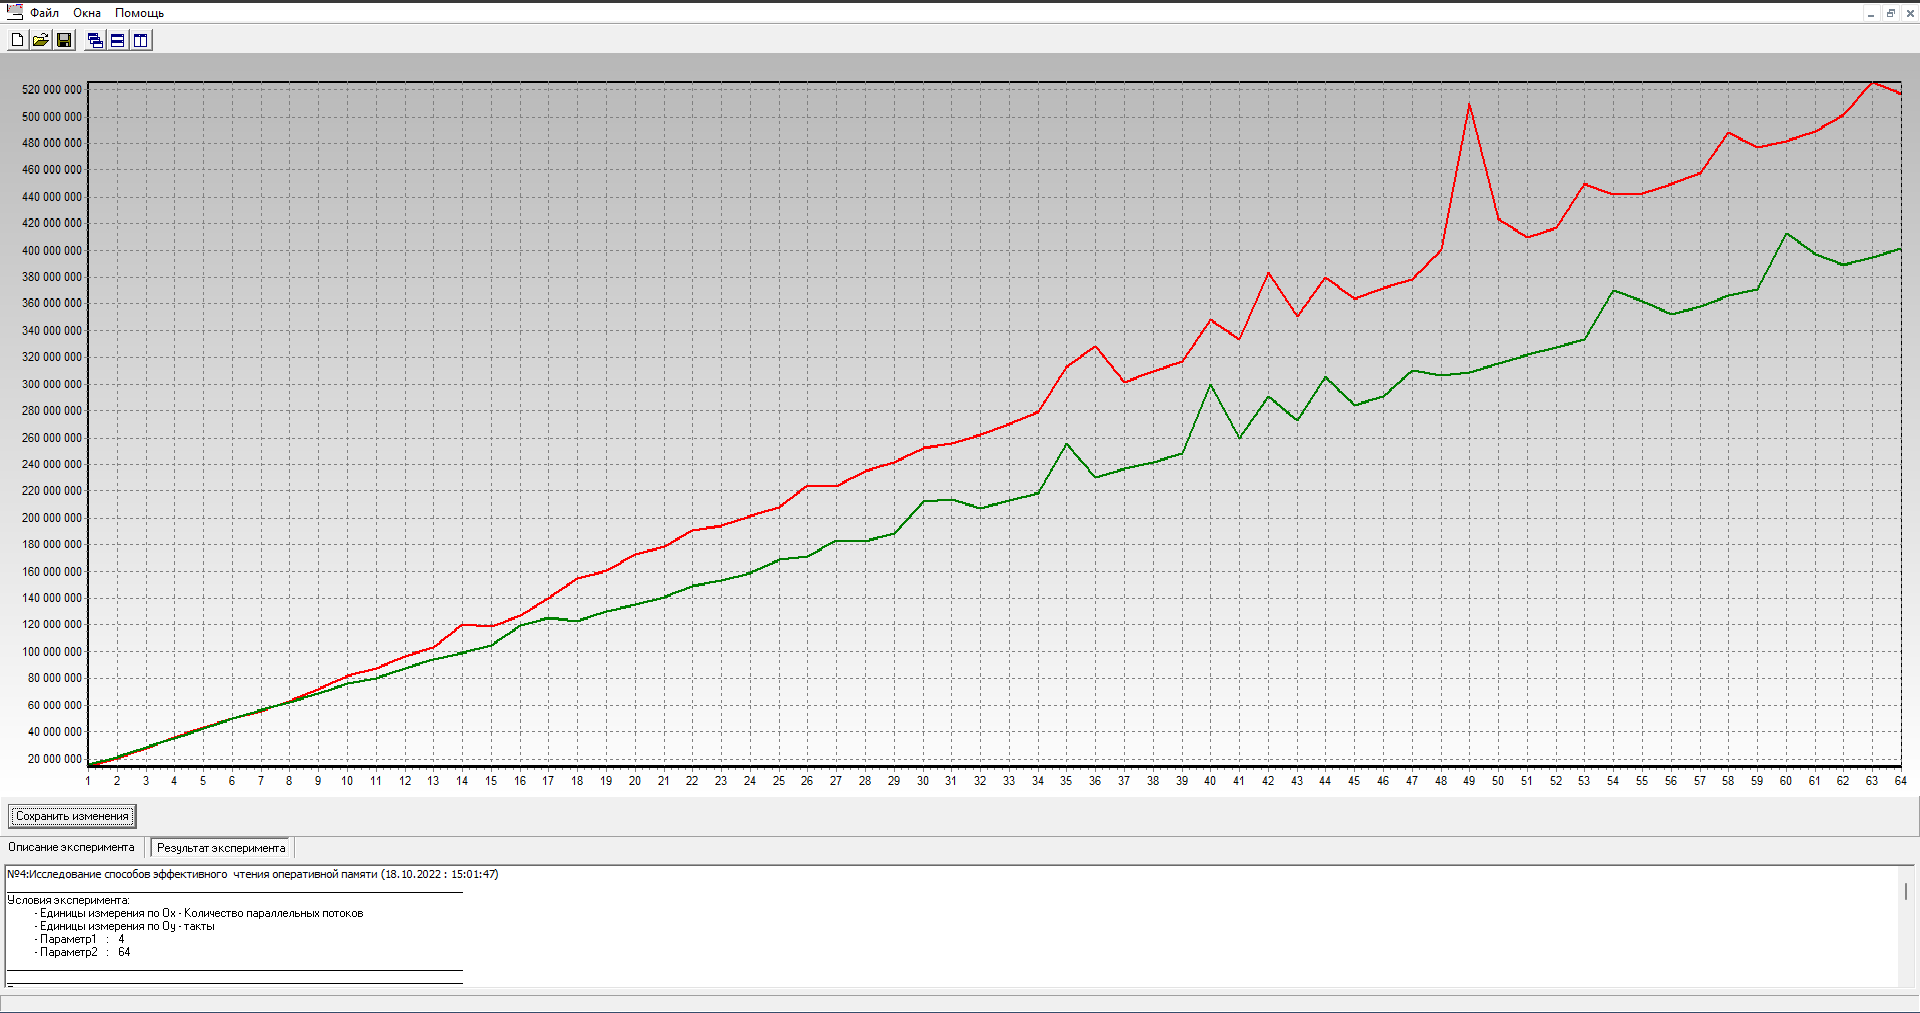
\includegraphics[height=0.35\textheight]{img/t4}
	\caption{Эксперимент №4: Исследование способов эффективного чтения оперативной памяти}
	\label{ex:t4}
\end{figure}

Результат сравнения времени (как вывод программы) представлен на
рисунке \ref{ex:t4-data}. Как видно на рисунке, неоптимизированная структура обрабатывалась в 1,2615723 раз дольше.

\begin{figure}[h]
	\centering
	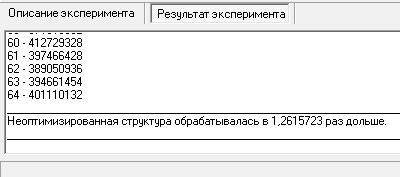
\includegraphics[height=0.15\textheight]{img/t4-data}
	\caption{Эксперимент №4: Результат}
	\label{ex:t4-data}
\end{figure}

Красный график показывает время или количество тактов работы алгоритма, использующего неоптимизированную структуру.

Зеленый график показывает время (или количество тактов) работы алгоритма с использованием оптимизированной структуры.

Оптимизация заключается в том, что структура данных, ускоряющая обработку современным процессорам, пытается максимально исключить несвоевременную передачу данных, то есть передавать только лишь востребованную для вычислений информацию. Поэтому снижается количество открытий и закрытий страниц DRAM-памяти и обеспечивается параллельная обработка данных, а также выполнение операций загрузки и выгрузки.

\subsection*{Вывод}
Можно сделать вывод, что для ускорения работы алгоритмов, необходимо правильно упорядочить данные.

\newpage

\section*{Эксперимент №5: Исследование конфликтов в кэш-памяти}
\addcontentsline{toc}{section}{Эксперимент №5}

\subsection*{Цель эксперимента}
Исследование влияния конфликтов кэш-памяти на эффективность вычислений.


\subsection*{Исходные данные}
Размер банка кэш-памяти данных первого и второго уровня, степень ассоциативности кэш-памяти первого и второго уровня, размер линейки кэшпамяти первого и второго уровня.

\subsection*{Описание проблемы}
Наборно-ассоциативная кэш-память состоит из линеек данных, организованных в несколько независимых банков. Выбор банка для каждой порции кэшируемых данных выполняется по ассоциативному принципу, т.е. из условия улучшения представительности выборки, в то время как целевая линейка в каждом из банков жестко определяется по младшей части физического адреса. Совокупность таких линеек всех банков принято называть набором. Таким образом, попытка читать данные из оперативной памяти с шагом, кратным размеру банка, приводит к их помещению в один и тот же набор.Если же количество запросов превосходит степень ассоциативности кэш-памяти, т.е. количество банков или количество линеек в наборе, то наблюдается постоянное вытеснение данных из кэш-памяти, причем больший ее объем остается незадействованным. 

\subsection*{Результаты эксперимента}
На рисунке \ref{ex:t5} предаставлен график, полученный в результате эксперимента с исходными параметрами:
\begin{itemize}
	\item Размер банка кэш-памяти (К) = 16;
	\item Размер линейки кэш-памяти (б) = 64;
	\item Количество читаемых линеек = 128.
\end{itemize}

\begin{figure}[h]
	\centering
	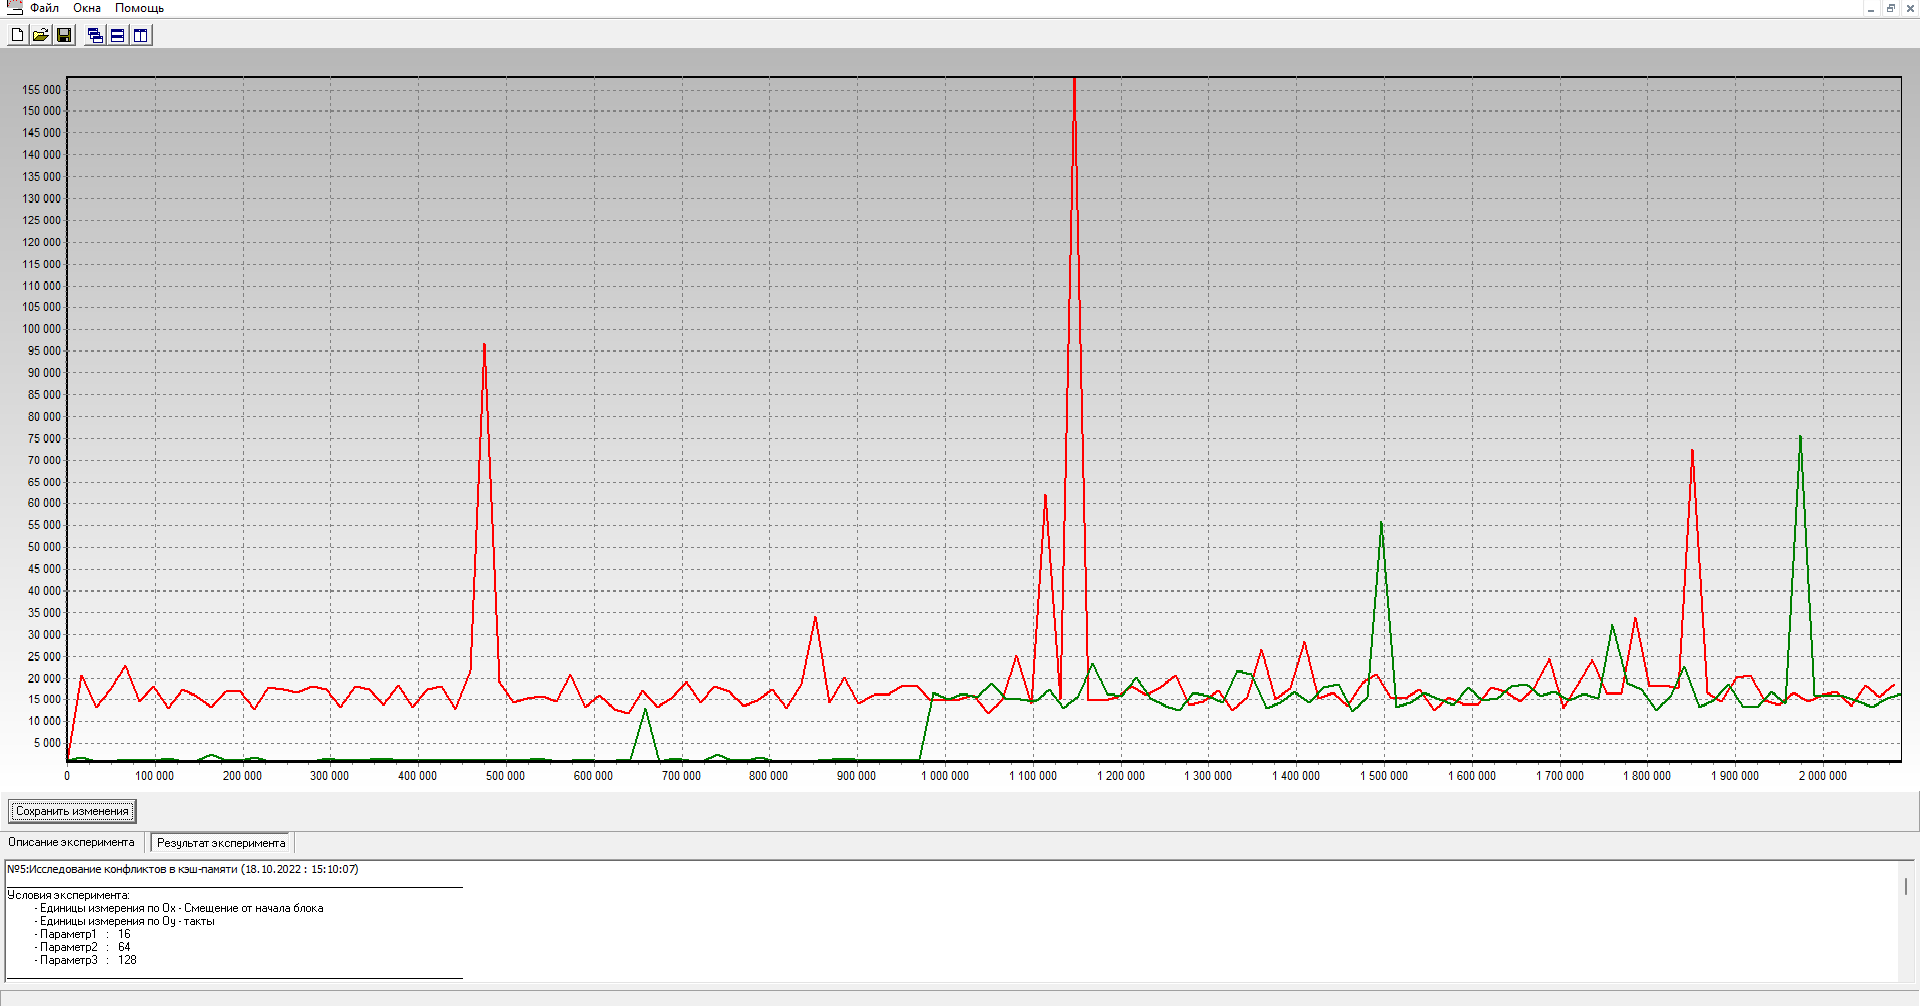
\includegraphics[height=0.35\textheight]{img/t5}
	\caption{Эксперимент №5: Исследование конфликтов в кэш-памяти}
	\label{ex:t5}
\end{figure}

Результат сравнения времени (как вывод программы) представлен на рисунке \ref{ex:t5-data}. Как видно на рисунке, чтение с конфликтами банков производилось в 1,9143146 раз дольше.

\begin{figure}[h]
	\centering
	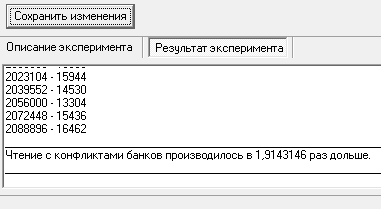
\includegraphics[height=0.15\textheight]{img/t5-data}
	\caption{Эксперимент №5: Результат}
	\label{ex:t5-data}
\end{figure}

Красный график показывает время или количество тактов работы процедуры, читающей данные с конфликтами в кэш-памяти. 

Зеленый график показывает время или количество тактов работы процедуры, не вызывающей конфликтов в кэш-памяти. Ось абсцисс отражает смещение читаемой ячейки от начала блока данных.

Красный график соответствует алгоритму, который построен таким образом, что чтение данных выполняется с шагом, кратным размеру банка. Именно это и порождает постоянные конфликты в кэш-памяти.

Зеленый график соответствует алгоритму, который оптимизируется размещение данных в кэш с помощью задания смещения востребованных данных на шаг, достаточный для выбора другого набора. (Шаг соответствует размеру линейки).

\subsection*{Вывод}
Можно сделать вывод, что использование кэш-памяти работа процессора ускоряется почти в 2 раз.

\section*{Эксперимент №6: Сравнение алгоритмов сортировки}
\addcontentsline{toc}{section}{Эксперимент №6}

\subsection*{Цель эксперимента}
Исследование способов эффективного использования памяти и выявление наиболее эффективных алгоритмов сортировки, применимых в вычислительных системах. 

\subsection*{Исходные данные}
Количество процессоров вычислительной системы, размер пакета, количество элементов в массиве, разрядность элементов массива.

\subsection*{Описание проблемы}
Существует несколько десятков алгоритмов сортировки. Их можно классифицировать по таким критериям, как: назначение (внутренняя и внешняя сортировки), вычислительная сложность (алгоритмы с вычислительными сложностями $O(n^2), O(n*log(n)), O(n), O(n/log(n))$), емкостная сложность (алгоритмы, требующие и не требующие дополнительного массива), возможность распараллеливания (не распараллеливаемые, ограниченно распараллеливаемые, полностью распараллеливаемые), принцип определения порядка (алгоритмы, использующие парные сравнения и не использующие парные сравнения).  

\subsubsection{Radix Sort}

Логика данной сортировки проста. Допустим, у нас есть массив из 10 чисел.

Сначала идет сортировка их по первому (старшему) разряду. Сортировка в таком случае выполняется с помощью сортировки подсчетом (count sort). Сложность — $O(n)$. 

В итоге получается 10 «корзин» — в которых старший разряд 0, 1, 2 и т.д.

Далее в каждой из корзин запускаем ту же процедуру, но только рассматриваем уже не старший разряд, а следующий за ним, и т.д.

Такие действия выполняется до последнего разряда.

\subsection*{Результаты эксперимента}
На рисунке \ref{ex:t6} предаставлен график, полученный в результате эксперимента с исходными параметрами:
\begin{itemize}
	\item Количество 64-х разрядных элементов массивов (М) = 10;
	\item Шаг увеличения размера массива (К) = 256.
\end{itemize}

\clearpage

\begin{figure}[h]
	\centering
	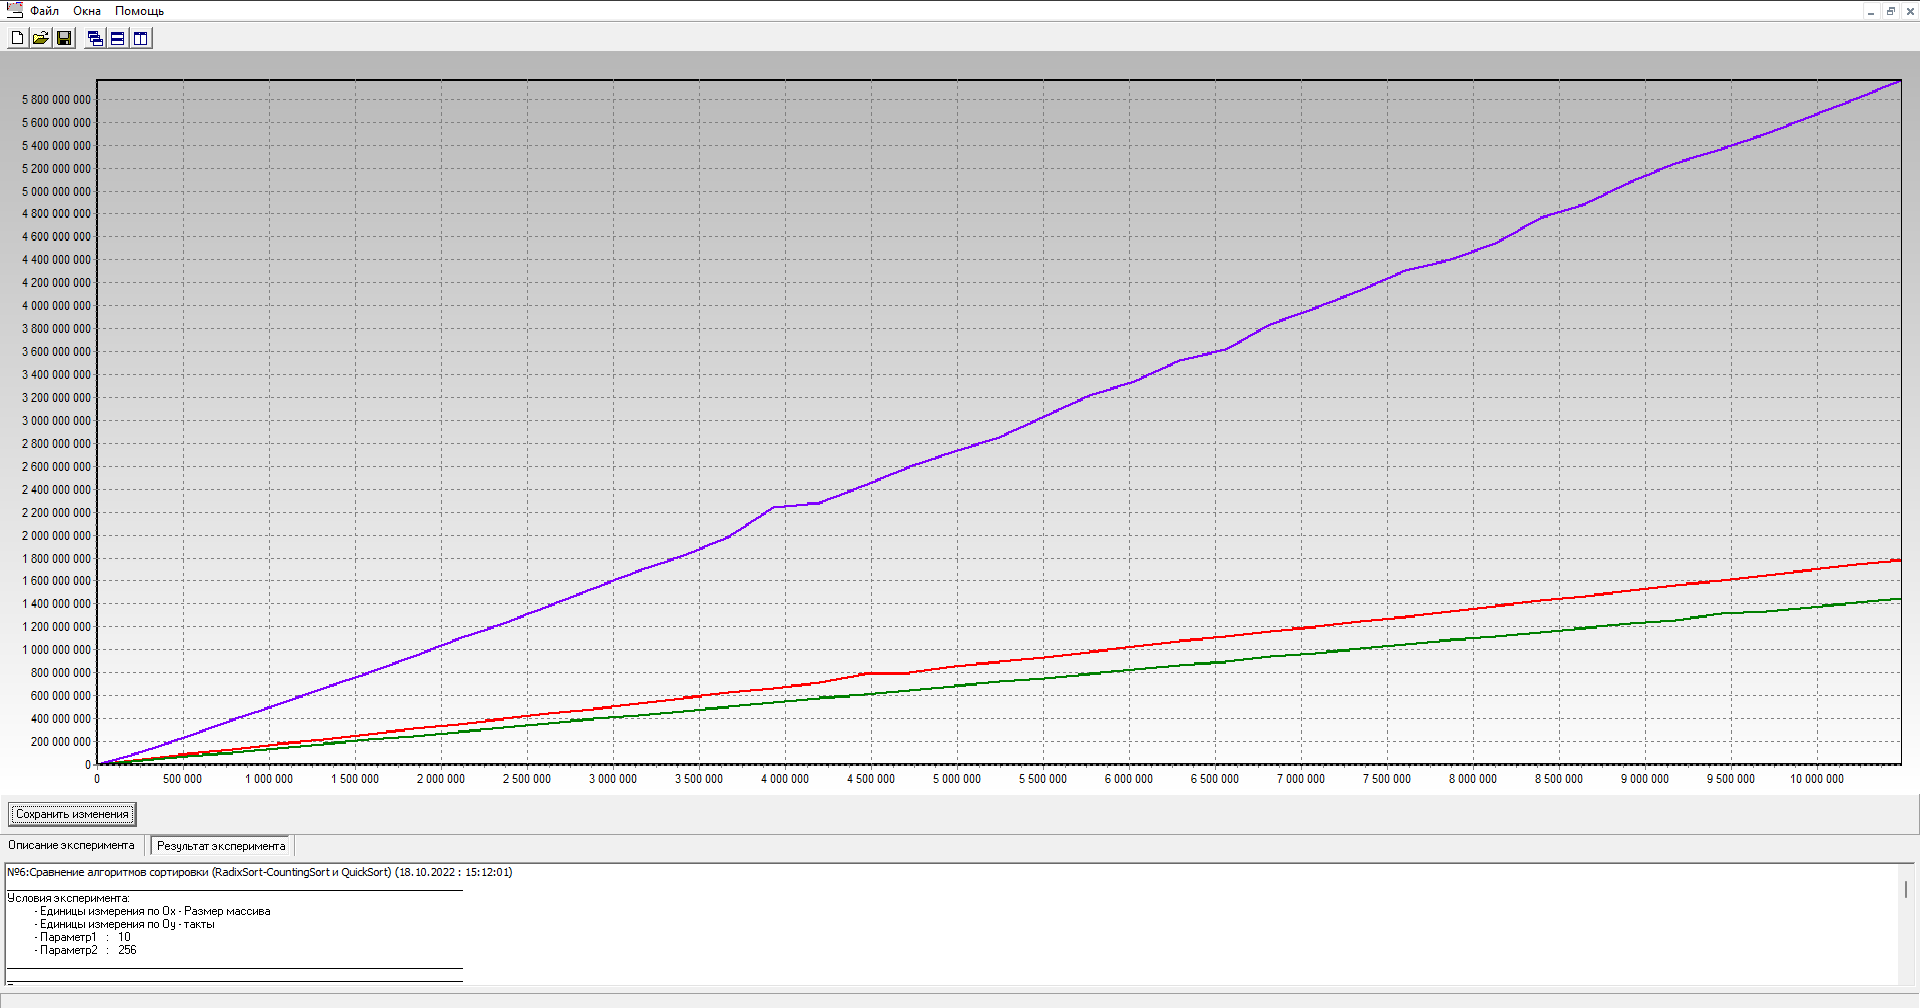
\includegraphics[height=0.35\textheight]{img/t6}
	\caption{Эксперимент №6: Сравнение алгоритмов сортировки}
	\label{ex:t6}
\end{figure}

Результат сравнения времени (как вывод программы) представлен на рисунке \ref{ex:t6-data}. Как видно на рисунке, QuickSort работал в 3,2639058 раз дольше Radix-Counting Sort, и QuickSort работал в 4,0400361 раз дольше Radix-Counting Sort, оптимизированного под 8-процессорную ЭВМ.

\begin{figure}[h]
	\centering
	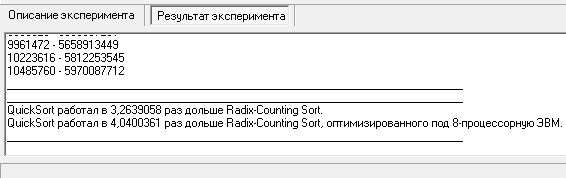
\includegraphics[height=0.15\textheight]{img/t6-data}
	\caption{Эксперимент №6: Результат}
	\label{ex:t6-data}
\end{figure}

Фиолетовый график показывает время или количество тактов работы алгоритма QuickSort. 

Красный график показывает время или количество тактов работы неоптимизированного алгоритма Radix-Counting. 

Зеленый график показывает время или количество тактов работы оптимизированного под 8-процессорную вычислительную систему алгоритма Radix-Counting.

\subsection*{Вывод}
Можно сделать вывод о том, что существует сортировка, работающая быстрее чем QuickSort, при этом, даже ее можно еще оптимизировать для более быстрой работы.

\chapter*{Контрольные вопросы}
\addcontentsline{toc}{chapter}{Контрольные вопросы}

\subsubsection{1. Назовите причины расслоения оперативной памяти.}

Скорость обработки данных в процессоре в несколько раз превышает скорость доступа к информации, которая размещена в оперативной памяти. Необходимо, чтобы итоговая скорость выполнения команды процессором как можно меньше зависела от скорости доступа к коду команды и к используемым в ней операндам из памяти. 

Расслоение ОЗУ — один из аппаратных путей решения проблемы дисбаланса в скорости доступа к данным, размещенным в оперативной памяти, и производительностью процессора.

Физически ОЗУ представимо в виде объединения k устройств, способных хранить одинаковое количество информации и способных взаимодействовать с процессором независимо друг от друга. При этом адресное пространство организовано таким образом, что подряд идущие адреса, или ячейки памяти, находятся в соседних устройствах (блоках) оперативной памяти. Тем самым расслоение памяти в идеале увеличивает скорость доступа в k раз, плюс буфер команд позволяет сократить обращения к ОЗУ.

Поэтому можно сказать, что ОЗУ без расслоения памяти — один контроллер на все банки, но ОЗУ с расслоением памяти — каждый банк обслуживает отдельный контроллер.

\subsubsection{2. Как в современных процессорах реализована аппаратная предвыборка.}

Аппаратная предвыборка происходит неявно, без участия программиста или компилятора. Кэш-контроллер анализирует, по каким адресам и в каком порядке программа обращается к оперативной памяти, и пытается предугадать, какие данные вскоре могут понадобиться программе, и осуществляет их автоматическую предвыборку в кэш-память.

Разумеется, по последовательности обращений программы в оперативную память в общем случае невозможно предсказать, какие данные понадобятся впоследствии.

Например, обработка массива: если кэш-контроллер обнаруживает, что оперативная память последовательно опрашивается с некоторым фиксированным шагом, то он делает предположение, что это проиходит обработка массива, и начинает загружать следующие блоки данных заранее.

Аппаратная предвыборка данных в кэш-память не застрахована от ошибок. Если кэш-контроллер распознал, что это не обход массива, то данные, которые он загрузит в кэш-память, могут и не понадобиться. Однако хуже ошибки может быть то, что они могут «вытеснить» какие-либо полезные данные, находившиеся в кэш-памяти, и их придется загружать еще раз. 

\subsubsection{3. Какая информация храниться в TLB.}
TLB (Translation-Lookaside Buffer) представляет собой память с ассоциативной выборкой, которая содержит 20-тиразрядные базовые адреса 32-х страниц, то есть, старшие 20 разрядов физического адреса страницы. Каждый из базовых адресов имеет свой признак (тег). В качестве тега используются старшие 20 разрядов линейного адреса, то есть поля TABLE и PAGE.

Случай, когда базовый адрес страницы находится в TLB, называется КЭШ-попаданием. 

Помимо тега для каждого базового адреса страницы в TLB хранится дополнительная информация, позволяющая определить, какую страницу можно заменить на вновь вводимую. Поскольку TLB хранит адреса только 32 страниц объема 4 кб каждая, то микропроцессор может непосредственно формировать физические адреса для 128 Кб памяти.

\subsubsection{4. Какой тип ассоциативной памяти используется в кэш-памяти второго уровня современных ЭВМ и почему.}

В современных компьютерах применяют кэш-память второго уровня, которая находится между процессором и ОП и еще больше повышает производительность ЭВМ.

Кэш-память 2-го уровня, как правило, унифицирована, т. е. может содержать как команды, так и данные.

Если она встроена в ядро ЦП, то говорят о S-cache (Secondary Cache, вторичный кэш), в противном случае -- о B-cache (Backup Cache, резервный кэш). В современных серверных ЦП объем S-cache составляет от одного до нескольких мегабайт, a B-cache -- до 64 Мбайт. 

\subsubsection{5. Приведите пример программной предвыборки.}

При программной предвыборке программист или компилятор явно вставляет в программу команды предвыборки данных по тому или иному адресу в оперативной памяти. 

Программные предвыборки потребляют ресурсы в процессоре, и использование слишком многих предвыборок может ограничить их эффективность. 

Примеры таких предвыборок -- предвыборку данных в цикле для независимости от информации находящейся вне цикла и предвыборку в основных блоках, которые часто исполняются, но которые редко используют ее не зависимо от целей предвыборки.